\chapter{PROJECTO}
\section{Hardware}
Para o desenvolvimento deste projeto, foi criado um kit de desenvolvimento para facilitar sua implementação, testar, efetuar alterações e melhoramentos.\\
\\
Abaixo pode-se ver a montagem em esqueleto do equipamento utilizado.
\newline
\\
\\
\begin{figure}[H]
	\centering
	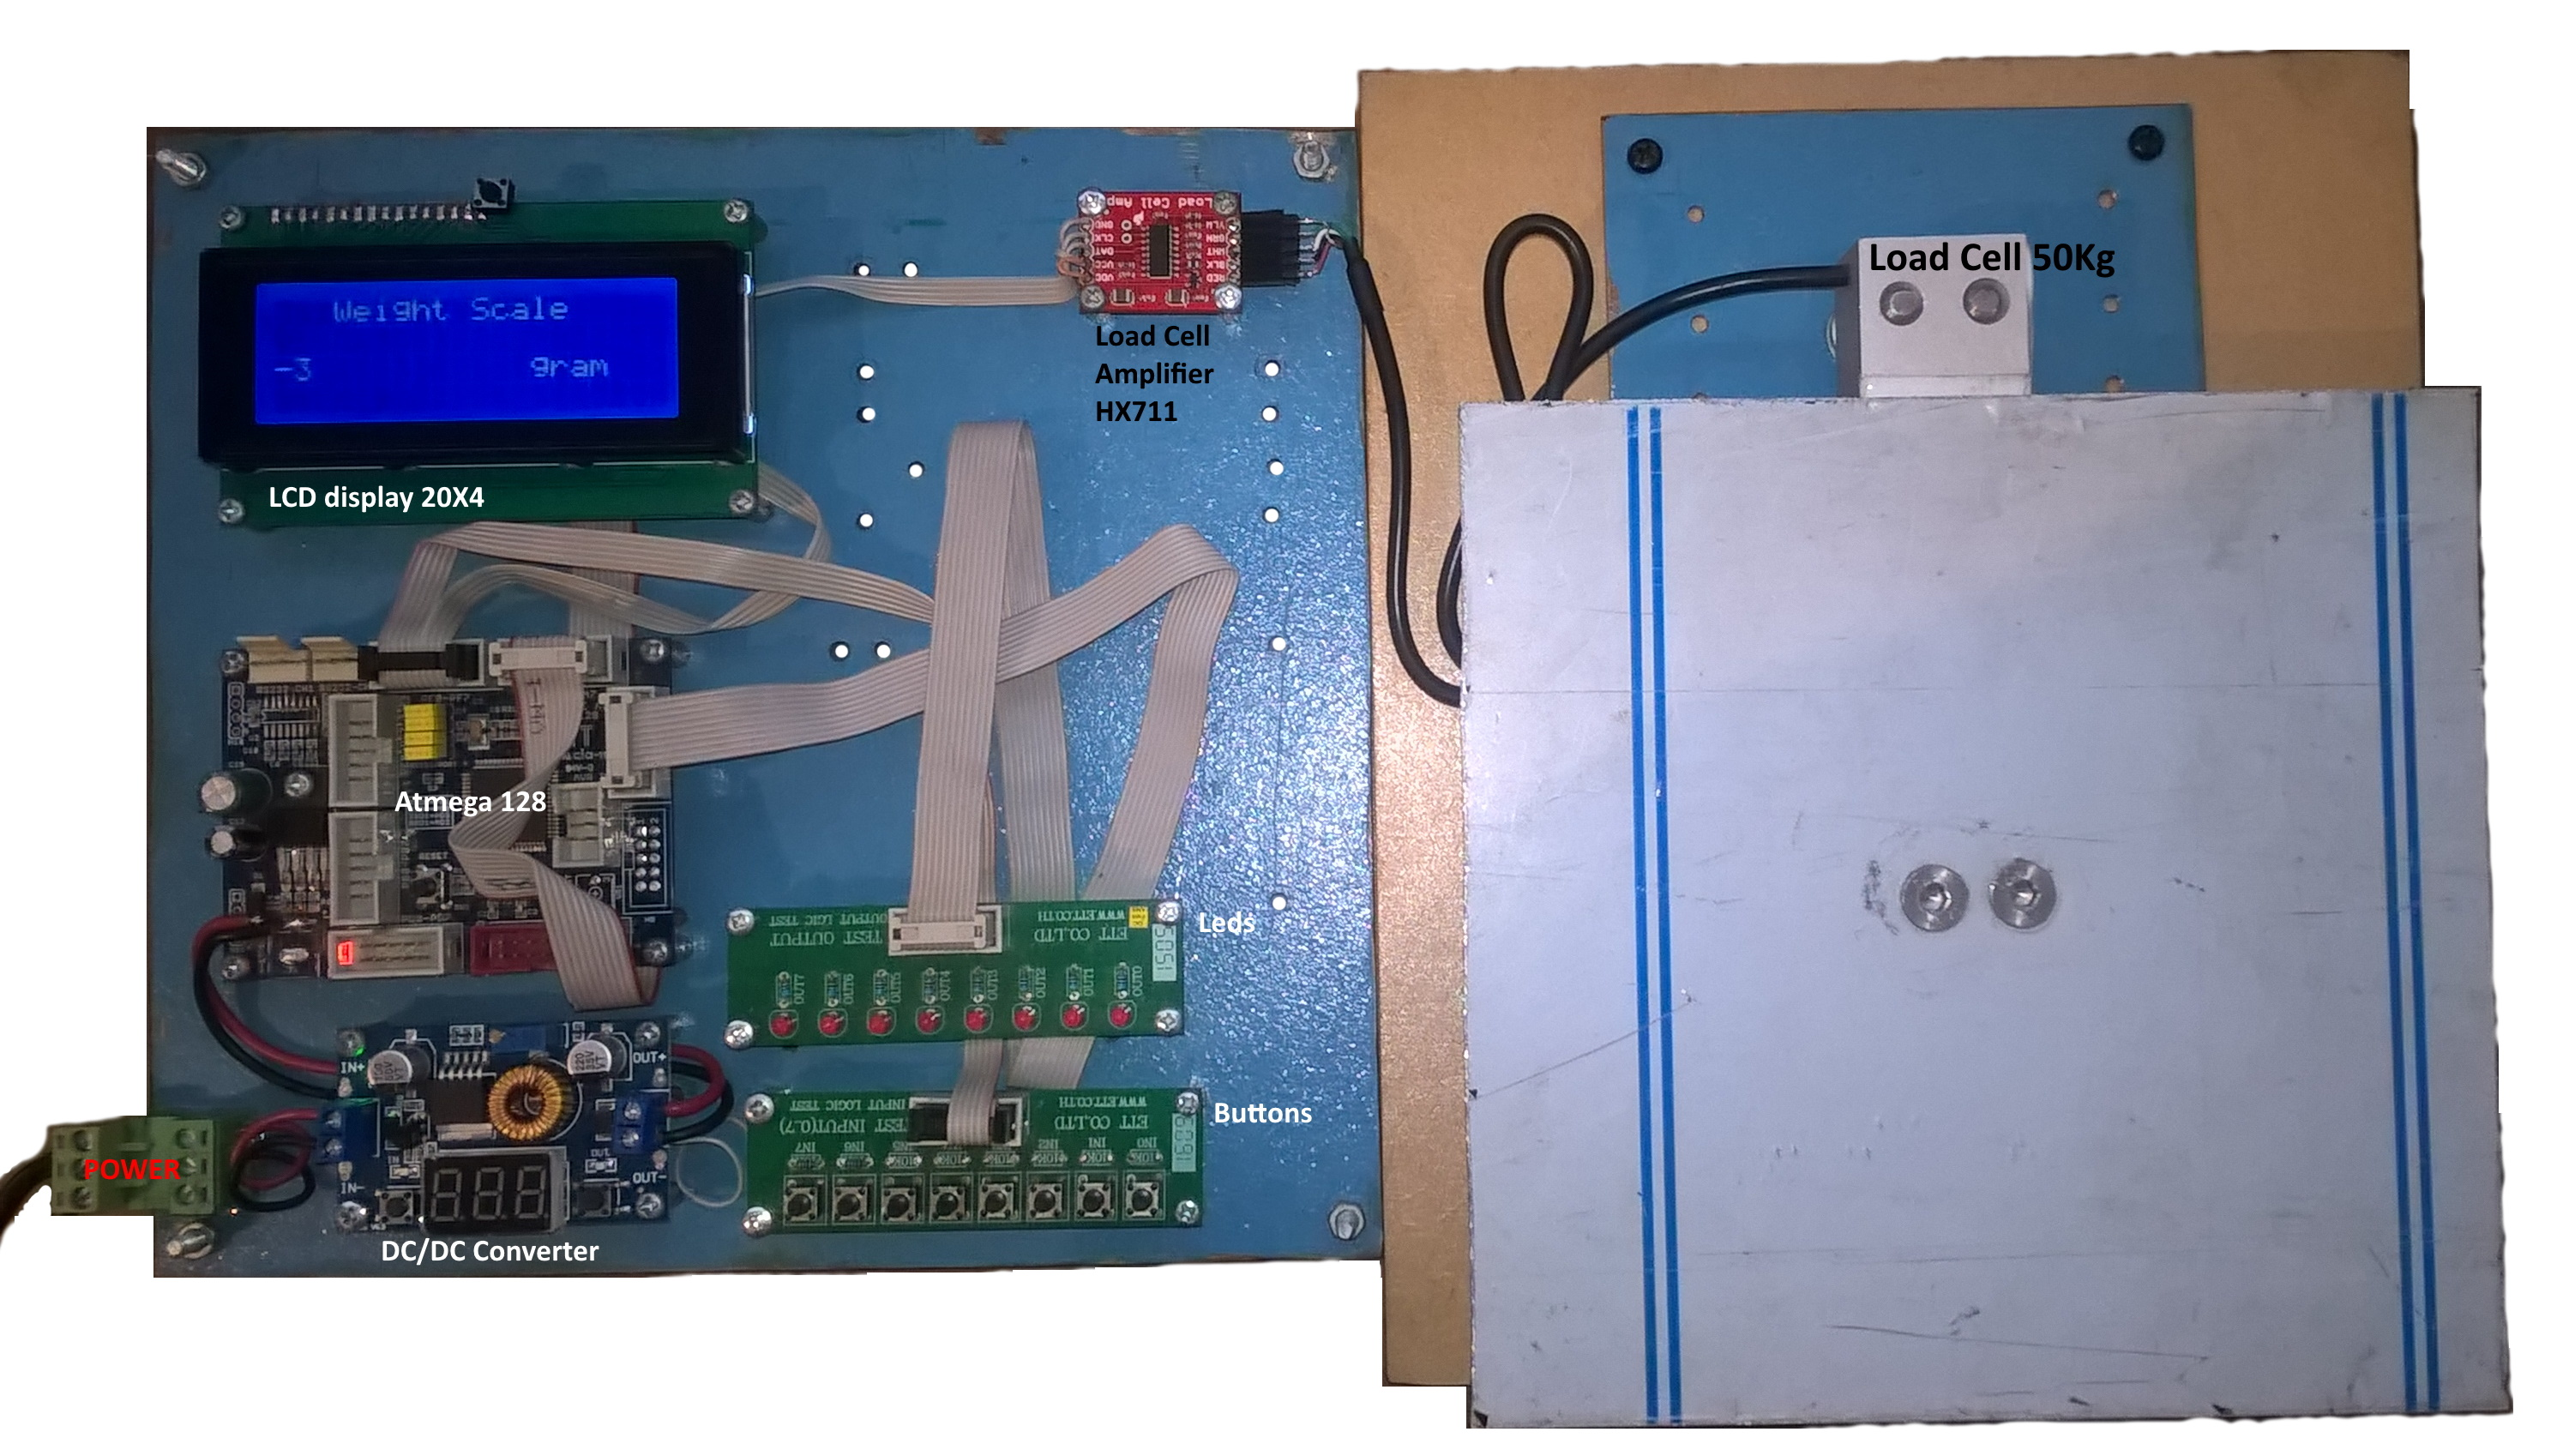
\includegraphics[scale=0.15]{./image/PESTA/kit/Kit_Desenvolvimento_2.jpg}
	\caption{Kit de Desenvolvimento}
	\label{Kit_Desenvolvimento_2}
\end{figure}
Para programar este microcontrolador (\textbf{Atmega 128}) foi utilizado o programador da marca da Atmel precisamente o \textbf{Atmel-ICE}, que para este equipamento tem disponível programação via ISP e JTAG.
\newpage
A montagem da mesa de medição,
\begin{figure}[H]
	\centering
	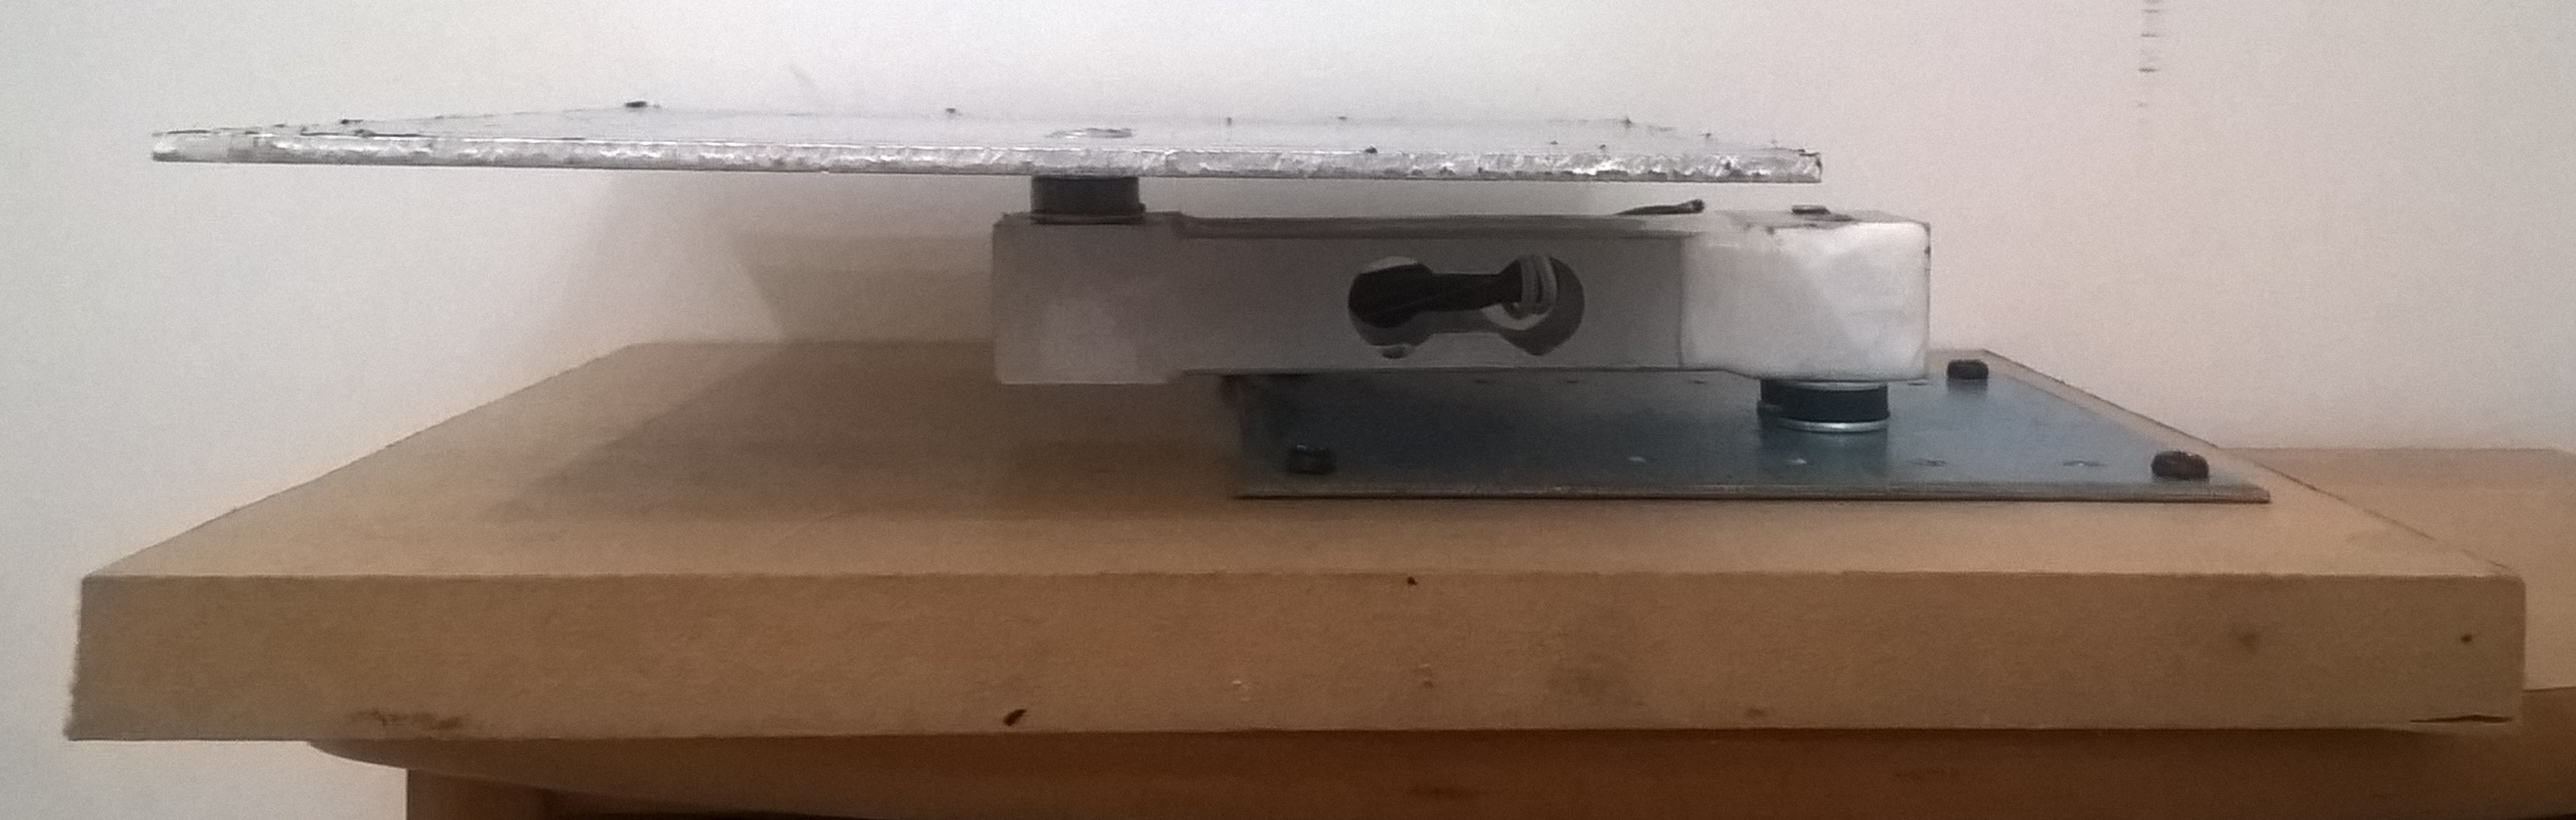
\includegraphics[scale=0.15]{./image/PESTA/material/Prato.jpg}
	\caption{Prato}
	\label{Prato}
\end{figure}
\subsection{Material}
Abaixo esta indicado uma tabela dos materiais usados, assim como os preços. 
\begin{table}[H]{
		\caption{Lista de material}
		\rowcolors{3}{blue!80!yellow!50}{blue!70!yellow!40}
		\begin{tabular}{ |p{12cm}|c|p{2cm}|  }
			\hline
			\multicolumn{3}{|c|}{Lista de Material} \\
			\hline
			Peça & Quant & Preço [uni] \\
			\hline
			Fonte de alimetação 12V 1A & 1 & \EUR{3.87} \\
			Conversor DC-DC com voltímetro & 1 & \EUR{7.75} \\
			ET BASE AVR Atmega128 Board & 1 & \EUR{23.92} \\
			Test Input Board  & 1 & \EUR{3.71} \\
			Test Output Board & 1 & \EUR{3.71} \\
			IDC Socket 10 way    & 12 & \EUR{0.31} \\
			IDC Header Straight 10 way    & 12 & \EUR{0.25} \\
			Flatcable    & ? & \EUR{?} \\
			20x4 LCD Module Blue & 1 & \EUR{12.24} \\
			SparkFun Load Cell Amplifier HX711 & 1 & \EUR{13.04}   \\
			50Kg Load Cell & 1 & \EUR{12} \\
			\hline
			 & \textit{total} & \EUR{86.96} \\
			\hline
		\end{tabular}
	}
	\label{material}
\end{table}
\newpage
\section{Funcionamento}
A ligação destes componentes é intuitivo e fácil de se perceber, o que é complexo neste trabalho é a interligação destes equipamentos com o micro-controlador por meio de \textit{software} e criar o \textit{driver} de comunicação para a placa do amplificador de sinal, já que o protocolo de comunicação é proprietário.
\begin{figure}[H]
	\captionsetup{justification=raggedright,singlelinecheck=false}
	\centering
	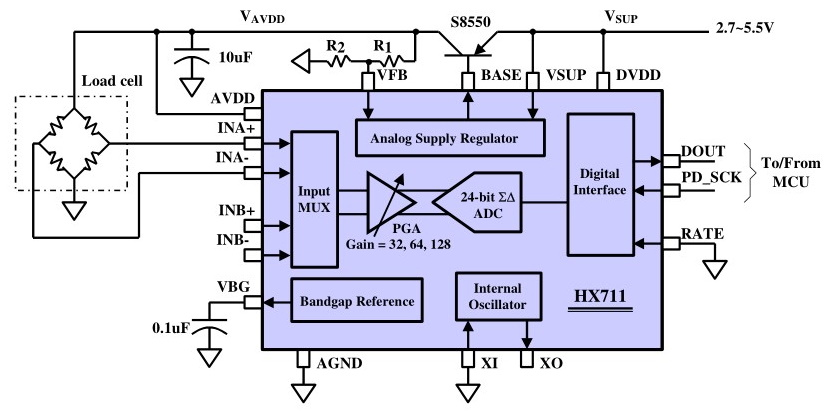
\includegraphics[scale=0.35]{./image/PESTA/schematic/HX711_Schematic_1.jpg}
	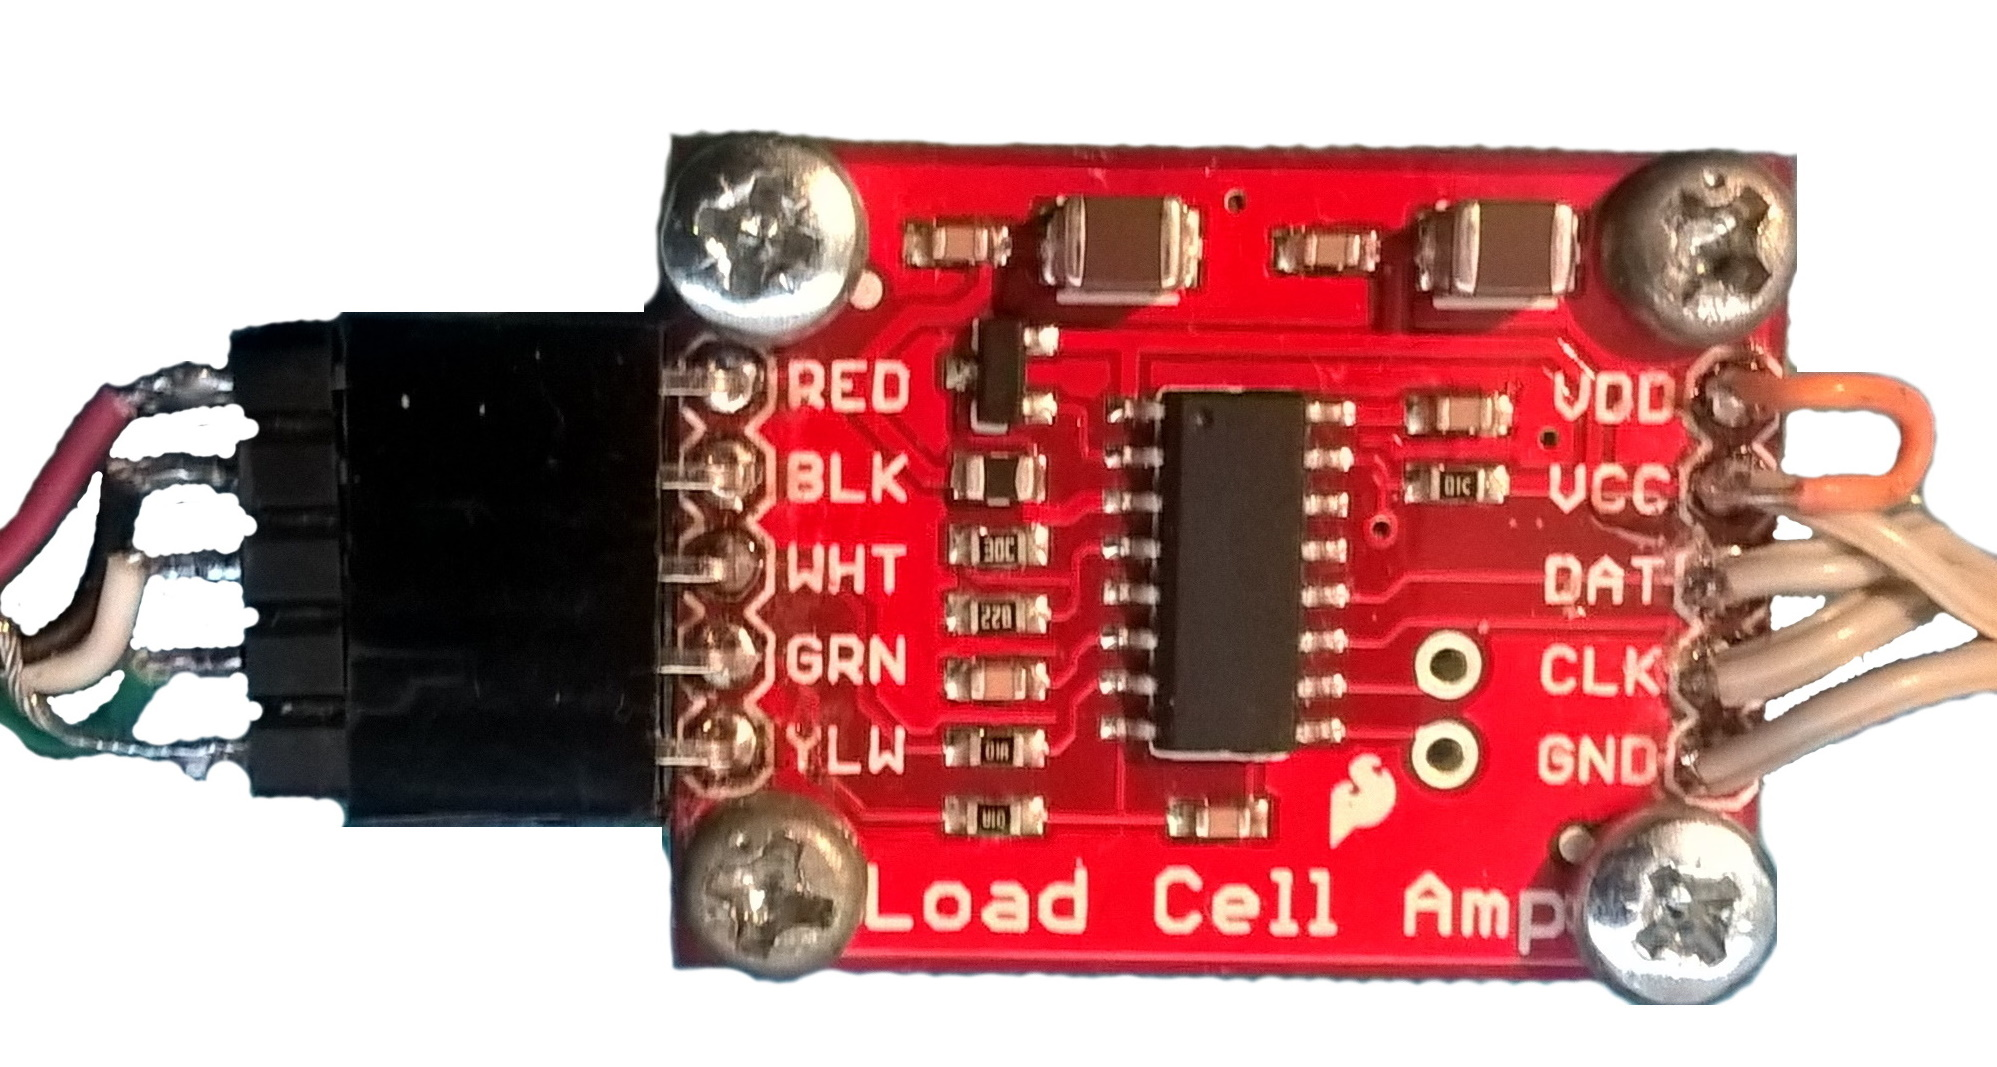
\includegraphics[scale=0.1]{./image/PESTA/material/HX711_board_1.jpg}
	\caption{Amplificador de Sinal [HX711]}
	\label{HX711_Schematic_1}
\end{figure}
A placa \textit{Load Cell Amplifier }pode ser programada fisicamente para determinar o numero de amostras por segundo a ser transmitido, tem opção de \textcolor{blue}{10} amostras por segundo e \textcolor{blue}{80} amostras, neste projeto optei pela segunda opção que necessita alteração na placa de circuito de impresso, isto é, abrir o \textit{jumper} respetivo de configuração.
\begin{figure}[H]
	\centering
	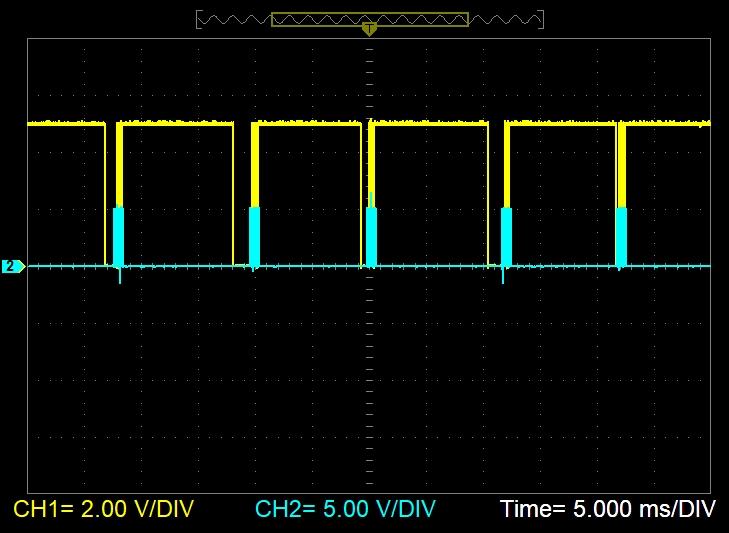
\includegraphics[scale=0.55]{./image/PESTA/graph/80SPS64GAIN/SPS_80.JPG}
	\caption{Amostras}
	\label{SPS_64}
\end{figure}
A livraria (driver) criada recorre a interrupções periódicas quando o sinal de \textit{data} vai para a massa, indicando assim que tem um pacote de leitura pronto a ser transmitido.\\
\\
%%\begin{minipage}{\linewidth}
\begin{minipage}[!b]{.40\linewidth}
	\begin{table}[H]
		\captionsetup{justification=raggedright,singlelinecheck=false}
		\caption{Configuração Ganho}
		\begin{tabular}{ | c | c | c |  }
			\hline
			\makecell[c]{PD\_SCK \\ Impulsos} & Entrada  & Ganho \\
			\hline
			\hline
			25 & \textbf{A} & 128 \\
			\hline
			26 & \textbf{B} & 32 \\
			\hline
			27 & \textbf{A} & 64 \\
			\hline
		\end{tabular}
		\label{Gain_Selection}
	\end{table}
	\vfill
\end{minipage}
\begin{minipage}[l]{.6\linewidth}
\vspace{.3cm}
Como indicado abaixo no gráfico em que a linha \textcolor{yellow}{amarela} é a informação e a linha \textcolor{BlueGreen}{azul} o respetivo \textit{clock} que é gerado pelas interrupções do micro-controlador fazendo \textit{shift} dos \textcolor{blue}{24} bits, que depois no fim transmite para o amplificador o ganho de amplificação a ser usado pelo numero excedente de \textit{clock cycles}, que nesta demonstração é \textcolor{blue}{um}, e corresponde a ganho de \textcolor{blue}{128}, respeitando a \textit{tabela} \ref{Gain_Selection}.
\end{minipage}\\
\\
%%\end{minipage}
\begin{figure}[H]
	\centering
	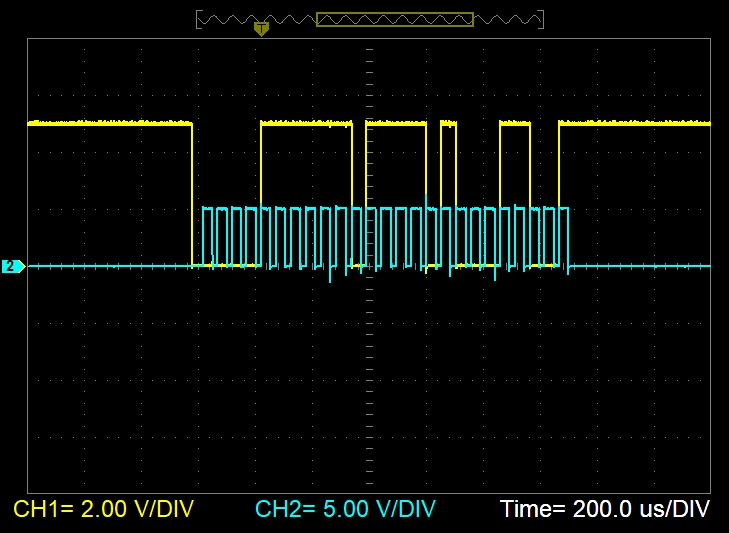
\includegraphics[scale=0.35]{./image/PESTA/graph/80SPS128GAIN/Gain_128_example.JPG}
	\caption{Ganho de 128}
	\label{Gain_128_example}
\end{figure}
a sequir o exemplo com o ganho de \textcolor{blue}{64}, pois tem \textcolor{blue}{três} impulsos excedentes.
\begin{figure}[H]
	\centering
	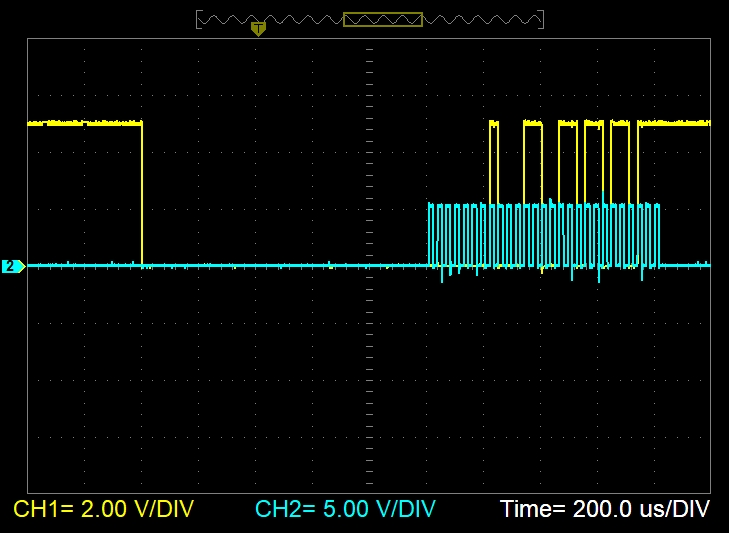
\includegraphics[scale=0.35]{./image/PESTA/graph/80SPS64GAIN/Gain_64_example.JPG}
	\caption{Ganho de 64}
	\label{Gain_64_example}
\end{figure}
Para obter este resultado a livraria driver para o \textit{Load Cell Amplifier} teve de ter em consideração que o microcontrolador é de \textcolor{blue}{8} bits, porque o pacote de informação consiste de \textcolor{blue}{24} \textit{bits} e em que é transmitido primeiro o \textit{bit} \textbf{MSB}.
\newpage
O codigo que executa esta rotina é demonstrado. \\
\begin{minipage}[l]{\linewidth}
\begin{minipage}[l]{.45\linewidth}
\begin{figure}[H]
	\flushleft
	\captionsetup{justification=raggedright,singlelinecheck=false}
	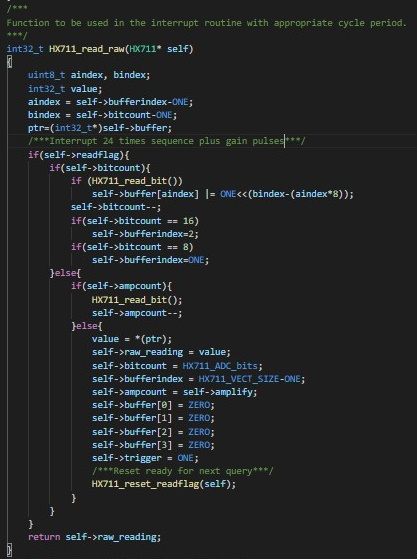
\includegraphics[scale=0.6]{./image/PESTA/Code/read_raw.jpg}
	\caption{Leitura ADC}
	\label{read_raw}
\end{figure}
\vspace{.7cm}
\end{minipage}
\begin{minipage}[l]{.35\linewidth}
\begin{figure}[H]
	\flushleft
	\captionsetup{justification=raggedright,singlelinecheck=false}
	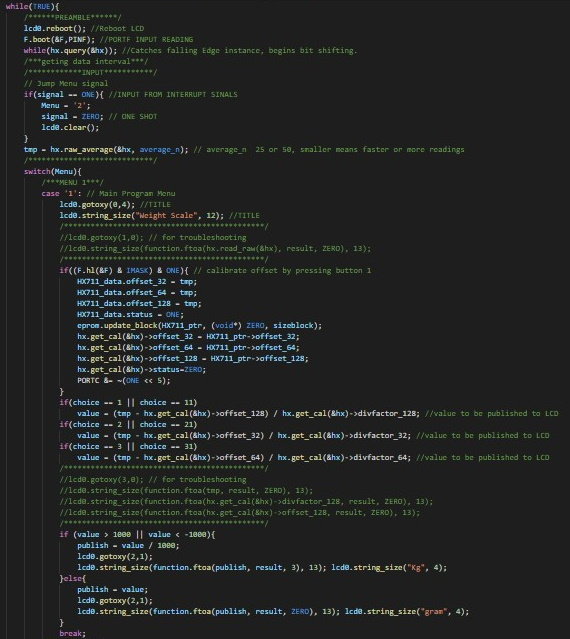
\includegraphics[scale=0.6]{./image/PESTA/Code/Main_While_Balanca.jpg}
	\caption{PROGRAM 1}
	\label{Main_While_Balanca}
\end{figure}
\end{minipage}
\end{minipage}
\newline
\vspace{.2cm}
\newline
Após obter um numero determinado de valores discretos é calculado sua média
\begin{equation}
	\label{eq:Mean}
	\overline{x}  =  \frac{1}{n}\sum_{i=1}^n x_i
\end{equation}
para ser tratado e deduzido o valor correspondente da massa.
\subsection*{Testar}
Quanto a funcionalidade no seu todo a balança tem \textcolor{blue}{quatro} botões e \textcolor{blue}{três} \textit{leds} ativados, um botão para fazer o \textit{offset} no \textcolor{green}{PORTF 0}, e dois botões com dupla função, fazer \textit{reset} para \textit{default} e incrementar, outro para entrar no menu de calibração e decrementar, o \textcolor{blue}{quarto} botão é reservado para \textit{enter} e assumir o valor introduzido na calibração.\\
\\
O botão \textcolor{green}{PORTF 3} quando premido durante \textcolor{blue}{cinco} segundos faz um \textit{reset} para configuração \textit{default} depois de o \textit{led} no \textcolor{red}{PORTC 6} piscar \textcolor{blue}{quatro} vezes.\\
\\
O botão \textcolor{green}{PORTF 4} quando premido durante \textcolor{blue}{cinco} segundos entra no menu de calibração do valor do \textit{gain factor} e o \textit{led} no \textcolor{red}{PORTC 7} liga, usando os botões de incrementa e decrementar, isto é, o
\textcolor{green}{PORTF 3} e \textcolor{green}{PORTF 4} pode-se alterar esse valor.\\
\\
Para assumir o valor e sair do menu de calibração basta premir o botão colocado no \textcolor{green}{PORTF 5}. Tanto no caso de calibração ou de \textit{offset} os valores são guardados na \textbf{EEPROM} do microcontrolador, sendo que, se retirar a alimentação do circuito este não perde os valores e o \textit{led} \textcolor{red}{PORTC 5} permanece ligado.
\newpage
\section{Software}
O \textbf{IDE} utilizado neste trabalho foi o \textbf{\textit{{Microchip Studio for AVR\textsuperscript{\textregistered} and SAM Devices}}} (\textit{version: 7.0.2542}). A programação foi feita em Linguagem \textbf{C}, sua estrutura sintática esta abaixo mencionado:
\begin{figure}[H]
	\centering
	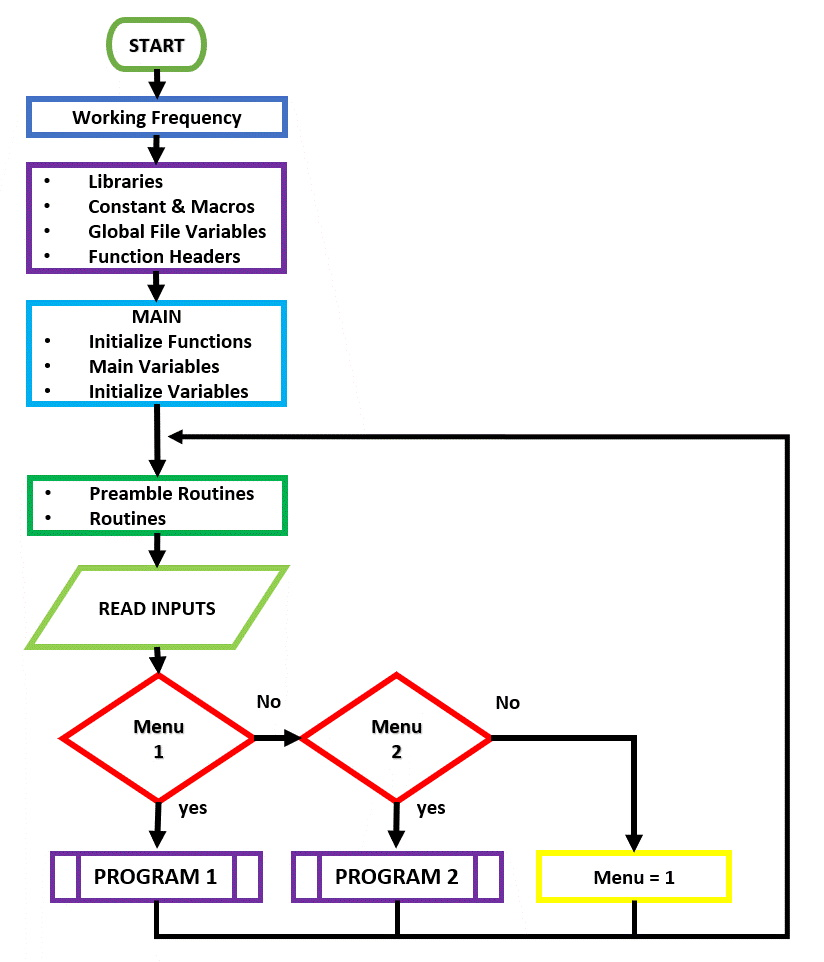
\includegraphics[scale=0.6]{./image/PESTA/flowchart/Main_Program_1.jpg}
	\caption{Estrutura do Programa}
	\label{Main_Program_1}
\end{figure}
O \textit{PROGRAM 1} é onde corre o programa da balança, e o \textit{PROGRAM 2} usado para calibração do \textit{Gain Factor}. \\
\newpage
Todos os programas sequem uma estrutura sintatica recursiva usando o seguinte modelo.
\begin{figure}[H]
	\centering
	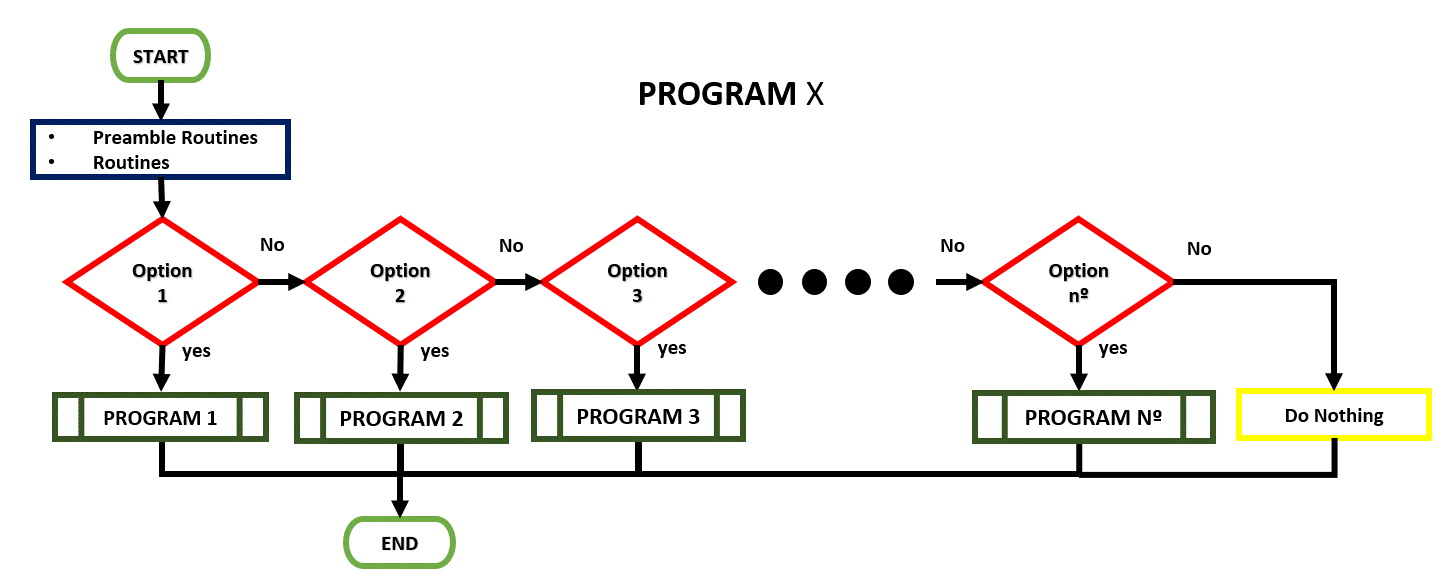
\includegraphics[scale=0.40]{./image/PESTA/flowchart/Generic_structure.jpg}
	\caption{Sintaxe Genérica dos programas}
	\label{Geneic_structure}
\end{figure}
Duas interrupções periódicas estão sempre a correr em \textit{background}, uma para fazer o \textit{shift} dos \textit{bit´s} da conversão \textbf{ADC} feita pelo amplificador de sinal HX711 e outra interrupção periódica de segundo em segundo usado para saltar de \textit{Menu} pelos botões.
\begin{minipage}{\linewidth}
\begin{minipage}{.5\linewidth}
\begin{figure}[H]
	\centering
	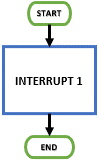
\includegraphics[scale=0.7]{./image/PESTA/flowchart/Interrupt_1.jpg}
	\caption{\textbf{ADC} conversão}
	\label{Interrupt_1}
\end{figure}
\end{minipage}
\begin{minipage}{.5\linewidth}
\begin{figure}[H]
	\centering
	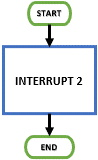
\includegraphics[scale=0.7]{./image/PESTA/flowchart/Interrupt_2.jpg}
	\caption{Saltar de \textit{Menu}}
	\label{Interrupt_2}
\end{figure}
\end{minipage}
\newline
\vspace{.1cm}
\newline
Consultar código para leitura das rotinas de interrupção nas folhas \textit{anexas}. \\
\end{minipage}
\begin{minipage}{.40\linewidth}
\begin{figure}[H]
	\flushleft
	\captionsetup{justification=raggedright,singlelinecheck=false}
	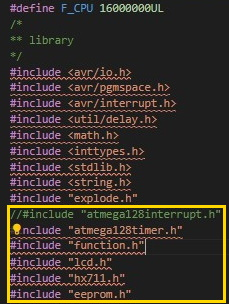
\includegraphics[scale=0.9]{./image/PESTA/Code/Livrarias.jpg}
	\caption{Livrarias}
	\label{Livrarias}
\end{figure}
\end{minipage}
\begin{minipage}{.6\linewidth}
Ao lado esta as livrarias usadas neste projeto, as que estão dentro da caixa amarela são as que foram criadas.
A filosofia usada é de criar objetos que representam o hardware para o poder manipular via código. Como se pode observar foi criado uma livraria para os temporizadores, outra paras as interrupções e \textbf{EEPROM} depois criado livrarias para os componentes externos, isto é, o \textbf{LCD} e o integrado \textbf{HX711}. \\
Uma abstração que torna simples executar qualquer algoritmo ou projeto, e isto só é possível depois de ultrapassar a barreira árdua e dolorosa de desenvolver as livrarias.\\
\\
\\
\end{minipage}
\newpage
\section{Validação}
%%%To validate is to justify why the choices made and alternatives that could be chosen.
As escolhas feitas estão dentro dos parâmetros da oferta disponibilizada. Apenas o conhecimento adquirido ao aprofundar o funcionamento dos componentes é o ganho mais evidente, facilitando a interpretação de situações e deteção de anomalias (\textit{troubleshooting}), derivado aos custos dos materiais serem caros.\\
\\
Apostei na marca \textbf{Atmel} devido a experiência e conhecimentos já adquiridos, se aposta-se noutra marca teria de enfrentar uma curva de aprendizagem e adaptação que no final a nível de custos beneficio seria desfavorável, pelo tempo a dispensar e de ser muito trabalhoso a refazer tudo novamente noutra arquitetura.\\
\\
O sensor usado é o mais comum nesta pratica, e escolha demonstrada, o circuito de interface é indiferente a escolha apenas é baseada na sua precisão, ou seja, é de \textcolor{blue}{24} \textit{bit} enquanto o \textbf{ADC} do \textbf{MCU} de \textcolor{blue}{10} \textit{bit}.
%%%%%%%%%%%%%%%%%%%%%%%%%%%%%%%%%%%%%%%%%%%%%%%%%%%%%%%%%%%%%%%%
\begin{comment}
Sem contar com as despesas no equipamento para a programação do hardware que em principio só se gasta uma vez, isto é, se não se estragar. No caso do programador \textbf{Atmel-ICE} pode custar até \EUR{185.55}.\\
\\
É de ter em conta que os preços são \textbf{PVP}, que no caso se for preços comerciais são dez vezes inferior, e se for para produção em grande escala também tem descontos por quantidade.\\
$\begin{array}{l l l}
\text{Média} & & \\
\overline{x} & = & \frac{1}{n}\sum_{i=1}^n x_i
\end{array}$
MEMS devices and structures are fabricated using conventional integrated circuit
process techniques, such as lithography, deposition, and etching, together with a
broad range of specially developed micromachining techniques. \cite{book-9}
The three essential elements in conventional
silicon processing are deposition, lithography, and etching. \cite{book-9}
Sensitivity,Long-Term Drift e Temperature Effects (Span temperature hysteresis).
%\newline
%\vspace{.1cm}
%\newline
\end{comment}
%%%%%%%%%%%%%%%%%%%%%%%%%%%%%%%%%%%%%%%%%%%%%%%%%%%%%%%%%%%%%%%%